% This LaTeX was auto-generated from MATLAB code.
% To make changes, update the MATLAB code and export to LaTeX again.

\documentclass{article}

\usepackage[utf8]{inputenc}
\usepackage[T1]{fontenc}
\usepackage{lmodern}
\usepackage{graphicx}
\usepackage{color}
\usepackage{hyperref}
\usepackage{amsmath}
\usepackage{amsfonts}
\usepackage{epstopdf}
\usepackage[table]{xcolor}
\usepackage{matlab}

\sloppy
\epstopdfsetup{outdir=./}
\graphicspath{ {./labPdsch_images/} }

\begin{document}

\matlabtitle{Simulating the 5G NR PDSCH over a Fading Channel }


\vspace{1em}
\begin{par}
\begin{flushleft}
In this lab, we will build a simple transmitter and receiver for the 5G NR downlink data channel, called the Physical Downlink Shared Channel or PDSCH.  We will perform the downlink simulation over a fading channel.  Writing this simulation from scratch would be months of work given all the complexity of the NR standard.  However, in this lab, we will be able to use \href{https://www.mathworks.com/help/5g/index.htm}{MATLAB's 5G Toolbox} which has incredible functions to perform all the basic operations.  
\end{flushleft}
\end{par}

\begin{par}
\begin{flushleft}
In going through the lab, you will learn to:
\end{flushleft}
\end{par}

\begin{itemize}
\setlength{\itemsep}{-1ex}
   \item{\begin{flushleft} Describe and visualize the OFDM frame structure of the NR standard including slots, subframes, and frames in time and sub-carriers and resource blocks in frequency. \end{flushleft}}
   \item{\begin{flushleft} Configure an OFDM channel with the 5G Toolbox. \end{flushleft}}
   \item{\begin{flushleft} Create a mutli-path channel in frequency domain for the OFDM link. \end{flushleft}}
   \item{\begin{flushleft} Measure the variation in SNR over one slot and over multiple slots to determine the effects of fast and slow fading. \end{flushleft}}
   \item{\begin{flushleft} Configure a PDSCH transmission including its resource block allocation and MCS. \end{flushleft}}
   \item{\begin{flushleft} Use 5G Toolbox commands to compute the transport block size, and perform the transmit steps including scrambling, LDPC encoding, symbol mapping and resource mapping to the OFDM grid. \end{flushleft}}
   \item{\begin{flushleft} Use 5G Toolbox commands to perform the RX steps including resource extraction, MMSE equalization, LDPC decoding, and  \end{flushleft}}
\end{itemize}

\begin{par}
\begin{flushleft}
Some of the code in this lab is based on  \href{https://www.mathworks.com/help/5g/ug/nr-pdsch-throughput.html}{MATLAB's PDSCH throuhput demo}.  You will need to get the R2020B version of MATLAB's 5G Toolbox for the demo.  The Toolbox is rapidly evolving, and I have used some functions that are not available in R2020A.  Also, along with this file, you will see three other files:
\end{flushleft}
\end{par}

\begin{itemize}
\setlength{\itemsep}{-1ex}
   \item{\begin{flushleft} \texttt{FDChan.m}:  A class for frequency-domain channel simulation \end{flushleft}}
   \item{\begin{flushleft} \texttt{NRgNBTxFD.m}:  A class for NR gNB TX frequency-domain simulation \end{flushleft}}
   \item{\begin{flushleft} \texttt{NRUERxFD.m}:  A class for NR UE RX frequency-domain simulation \end{flushleft}}
\end{itemize}

\begin{par}
\begin{flushleft}
These files have some TODO sections to be completed.
\end{flushleft}
\end{par}

\begin{par}
\begin{flushleft}
\textbf{Submission}:  Complete this MATLAB live file and the other files.  Run the code.  Print all the files to PDF.  Merge to a single PDF and submit the PDF for grading.
\end{flushleft}
\end{par}


\matlabheading{5G NR OFDM Channel Background}

\begin{par}
\begin{flushleft}
One of the main goals of the 5G NR standard was to build a highly configurable channel structure that can operate in a range of frequencies and band allocations.  The figure below are taken from this excellent website: \href{https://www.rfwireless-world.com/5G/5G-NR-Numerology-or-Terminology.html}{https://www.rfwireless-world.com/5G/5G-NR-Numerology-or-Terminology.html} 
\end{flushleft}
\end{par}

\begin{par}
\begin{flushleft}
To enable configuration, the 5G NR standard uses OFDM with a configurable time and frequency structure.  For the time structure, time is divided into\textbf{ radio frames} of 10 ms, which are then divided into 10 \textbf{sub-frames} of 1ms each.  The subframes are then divided into \textbf{slots} where the number of slots per subframe are configurable.  Specifically, the NR channel has a basic \textbf{configuration parameter} \texttt{mu=0,1,...,4, }and the number of slots per subframe is \texttt{2\textasciicircum{}mu.  }
\end{flushleft}
\end{par}

\begin{par}
\begin{flushleft}
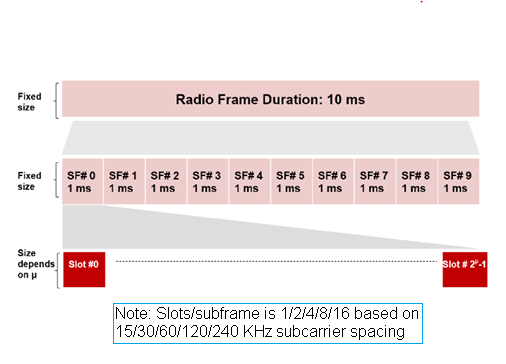
\includegraphics[width=\maxwidth{50.77772202709483em}]{image_0}
\end{flushleft}
\end{par}


\vspace{1em}
\begin{par}
\begin{flushleft}
In frequency, the channel uses OFDM with a sub-carrier spacing \texttt{Delta f,} that is tied to the configuration \texttt{mu.  }In each slot, the bandwidth is then divided into what are called \textbf{resource blocks} \textbf{(RBs) }which are 12 subcarriers for one slot.  The total bandwidth is then controlled by configuring the total number of resource blocks.  The sub-carrier spacing and the minimum and maximum number of RBs for each configuration \texttt{mu} is shown below.
\end{flushleft}
\end{par}


\vspace{1em}
\begin{par}
\begin{flushleft}
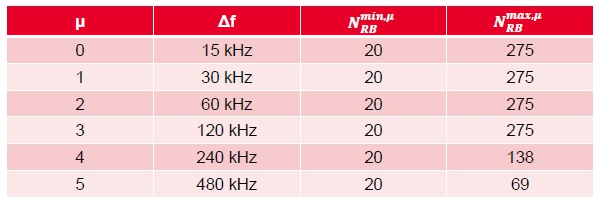
\includegraphics[width=\maxwidth{-0.10035122930255896em}]{image_1}
\end{flushleft}
\end{par}


\vspace{1em}
\begin{par}
\begin{flushleft}
Finally, each slot is divided into OFDM symbols.  The number of symbols per slot is 14 for what is called the normal cyclic prefix and 12 for extended cyclic prefix.  Most systems use normal CP.  The extended CP is used for environments with very large delay spreads.
\end{flushleft}
\end{par}

\begin{par}
\begin{flushleft}
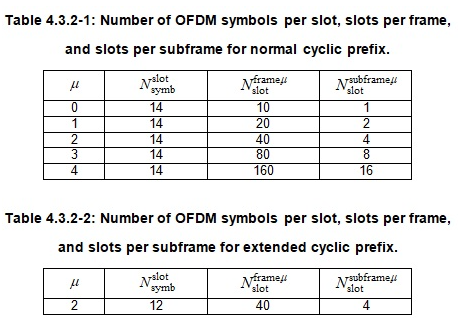
\includegraphics[width=\maxwidth{-0.10035122930255896em}]{image_2}
\end{flushleft}
\end{par}


\vspace{1em}

\matlabheading{Configuring the OFDM Channel}

\begin{par}
\begin{flushleft}
In this lab, we will configure the parameters for an OFDM channel at a carrier frequency of 28 GHz.  We will use the following parameters, which are widely-used in these frequencies.
\end{flushleft}
\end{par}

\begin{matlabcode}
fc = 28e9;                % Carrier frequency
SubcarrierSpacing = 120;  % SCS in kHZ
NRB = 66;  % number of resource blocks
\end{matlabcode}

\begin{par}
\begin{flushleft}
Using the SCS and number of resource blocks, compute and print the bandwidth occupied by this waveform.
\end{flushleft}
\end{par}

\begin{matlabcode}
nscPerRB = 12;  % number of sub-carriers per RB

% TODO:
bwMHz = SubcarrierSpacing * NRB * nscPerRB / 1e3;
fprintf(1, 'The bandwidth in [MHz] = %.2f\n', bwMHz);
\end{matlabcode}
\begin{matlaboutput}
The bandwidth in [MHz] = 95.04
\end{matlaboutput}


\begin{par}
\begin{flushleft}
In the 5G Toolbox, you can configure the channel with the \texttt{nrCarrierConfig} command which creates an object with all the relevant parameters.  Use the \texttt{nrCarrierConfig} command to create a \texttt{carrierConfig} structure with the \texttt{SubcarrierSpacing} from above and the property NSizeGrid set to \texttt{NRB}.
\end{flushleft}
\end{par}

\begin{matlabcode}
% TODO
carrierConfig = nrCarrierConfig("NSizeGrid",NRB,"SubcarrierSpacing",SubcarrierSpacing);
\end{matlabcode}


\begin{par}
\begin{flushleft}
Given the \texttt{carrierConfig} we can the configuration of the waveform with following command:
\end{flushleft}
\end{par}

\begin{matlabcode}
waveformConfig = nrOFDMInfo(carrierConfig);
\end{matlabcode}


\begin{par}
\begin{flushleft}
Use the \texttt{waveformConfig} structure to print:
\end{flushleft}
\end{par}

\begin{itemize}
\setlength{\itemsep}{-1ex}
   \item{\begin{flushleft} The sample rate in MHz \end{flushleft}}
   \item{\begin{flushleft} Number of OFDM symbols per subframe \end{flushleft}}
\end{itemize}

\begin{matlabcode}
% TODO
srMHz = waveformConfig.SampleRate / 1e6;
symbsSubframe = waveformConfig.SlotsPerSubframe * waveformConfig.SymbolsPerSlot;
fprintf(1, 'The sample rate in [MHz] = %.2f\n', srMHz);
\end{matlabcode}
\begin{matlaboutput}
The sample rate in [MHz] = 122.88
\end{matlaboutput}
\begin{matlabcode}
fprintf(1, 'The number of symbols per subframe = %.f\n', symbsSubframe);
\end{matlabcode}
\begin{matlaboutput}
The number of symbols per subframe = 112
\end{matlaboutput}


\matlabheading{Configuring a Frequency-Domain OFDM Channel}

\begin{par}
\begin{flushleft}
In this lab, we will simulate the channel in frequency domain.  For OFDM systems, frequency-domain simulation enables us to avoids the need to simulate the TX and RX filtering, synchronization and channel estimation.  We can add these components of the simulation later.  We will use the following simple channel with two paths.
\end{flushleft}
\end{par}

\begin{matlabcode}
% Parmaeters for each path
gain = [0,-3]';      % path gain in dB
dly = [0, 200e-9]';  % path delays in seconds
aoaAz = [0, 180]';  % angles of arrival
aoaEl = [0, 20]';

% Mobile velocity vector in m/s
rxVel = [30,0,0]';

% Parameters for computing the SNR
Etx = 1;        % Average transmitted symbol energy
EsN0Avg = 20;   % Average SNR
\end{matlabcode}

\begin{par}
\begin{flushleft}
The lab material contains a file, \texttt{FDChan.m} which has a skeleton for modeling channels in frequency domain.   You can create this channel object using this file with the following command:
\end{flushleft}
\end{par}

\begin{matlabcode}
fdchan = FDChan(waveformConfig, 'gain', gain, 'dly', dly, 'aoaAz', aoaAz, 'aoaEl', aoaEl, ...
                'rxVel', rxVel, 'Etx', Etx, 'EsN0Avg', EsN0Avg, 'fc', fc);
\end{matlabcode}


\begin{par}
\begin{flushleft}
The file \texttt{FDChan.m} has various sections labeled \texttt{TODO} that should be completed.  First, complete the section in the constructor that sets complex gains for each path
\end{flushleft}
\end{par}

\begin{par}
\begin{flushleft}
The vector \texttt{gainComplex} should have one complex value for each path, with the gain set by gaindB and a random complex phase from \texttt{[0,2*pi]} .
\end{flushleft}
\end{par}

\begin{par}
\begin{flushleft}
Next, set the Doppler for each path based on the mobile velocity and angles of the path. by completing the following part:
\end{flushleft}
\end{par}

\begin{par}
\begin{flushleft}
Edit the code, recreate the \texttt{fdchan} object and print the Doppler shifts:
\end{flushleft}
\end{par}

\begin{matlabcode}
% TODO:  Print fdchan.fd
fprintf(1, 'The Doppler shifts [Hz] = %.2f\n', fdchan.fd);
\end{matlabcode}
\begin{matlaboutput}
The Doppler shifts [Hz] = 2801.94
The Doppler shifts [Hz] = -2632.96
\end{matlaboutput}


\begin{par}
\begin{flushleft}
For the fd simulator, we will also need to compute the time of the OFDM symbols relative to the beginning of the sub-frame.  Complete the following section in the \texttt{FDChan} class to create a vector obj.symStart where `obj.symStart(i) is the time, in seconds, of the start of the \texttt{i}-th OFDM symbol relative to the beginning of the subframe.  You can use the waveformConfig.SymbolLengths and waveformConfig.SampleRate.  
\end{flushleft}
\end{par}

\begin{par}
\begin{flushleft}
 Plot \texttt{fdchan.symStart.  }If you did this correctly, the values should go from 0 to 1ms.
\end{flushleft}
\end{par}

\begin{matlabcode}
% TODO
symbStarts = fdchan.symStart;
figure;
stem(symbStarts*1e3);
xlabel("Symbol sequence number in the subframe"); ylabel("Start Time [ms]");
title("Start time for each symbol relative to the start of the subframe");
grid on;
\end{matlabcode}
\begin{center}
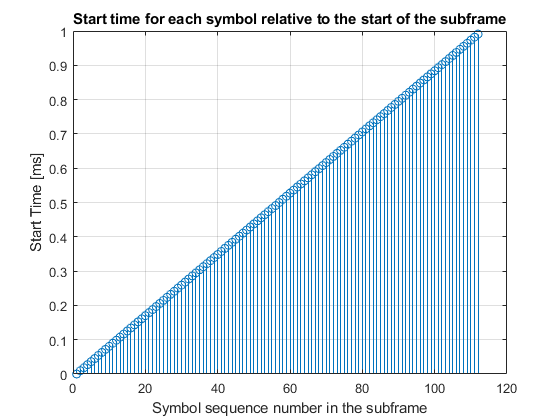
\includegraphics[width=\maxwidth{56.196688409433015em}]{figure_0.png}
\end{center}


\matlabheading{Simulating the Frequency-Domain Channel}

\begin{par}
\begin{flushleft}
The method, \texttt{FDChan.stepImpl()} takes as an input an array, \texttt{txGrid(n,j),} representing the TX OFDM data on sub-carriers \texttt{n} and OFDM symbol numbers j.  The output grid is given by,
\end{flushleft}
\end{par}

\begin{verbatim}
rxGrid(n,j) = chan(n,j)*txGrid(n,j) + noise(n,j)
\end{verbatim}
\begin{par}
\begin{flushleft}
where the channel is:
\end{flushleft}
\end{par}

\begin{verbatim}
chan(n,j) = \sum_k gainComplex(k)*exp(2*pi*1i*(time(j)*fd(k) + n*scs*dly(k))
\end{verbatim}
\begin{par}
\begin{flushleft}
and \texttt{time(j)} is the start time of the \texttt{j-}th symbol and \texttt{scs} is the sub-carrier spacing.  The noise variance is set to obtain a cerain average SNR  given by,
\end{flushleft}
\end{par}

\begin{verbatim}
EsN0Avg = Etx*E| chan(n,t) |^2 / noiseVar
\end{verbatim}
\begin{par}
\begin{flushleft}
The average channel gain is 
\end{flushleft}
\end{par}

\begin{verbatim}
E| chan(n,t) |^2 = \sum_k |gainComplex(k)|^2
\end{verbatim}
\begin{par}
\begin{flushleft}
Use these formulae to complete the method \texttt{stepImpl}.
\end{flushleft}
\end{par}

\begin{matlabcode}
% TODO:  Complete the method FDChan.stepImpl()
\end{matlabcode}


\begin{par}
\begin{flushleft}
To test the channel, we will create a TX grid corresponding to one slot.  You can do this with the following command.
\end{flushleft}
\end{par}

\begin{matlabcode}
NumLayers = 1;
txGrid = nrResourceGrid(carrierConfig, NumLayers);
txGrid(:) = 1;
\end{matlabcode}

\begin{par}
\begin{flushleft}
Use the \texttt{fdchan.step()} method to find the channel and noise variance on this grid at subframe number, \texttt{sfNum=0} and slot number, \texttt{slotNum=0}.  Compute the SNR in dB over the grid and plot the SNR using the \texttt{imagesc} command.  You should see there is a high level of variation of the SNR across the slot indicating significant \textbf{fast fading}.
\end{flushleft}
\end{par}

\begin{matlabcode}
% TODO
[rxGrid_test, chanGrid_test, noiseVar_test] = fdchan.step(txGrid, 0, 0);
nsc = NRB*12;
figure;
imagesc(1:14, 1:nsc, pow2db(abs(chanGrid_test).^2/noiseVar_test));
ylabel("Subcarrier Number"); xlabel("Symbol Number");
title("SNR [dB] over the grid");
colorbar();
\end{matlabcode}
\begin{center}
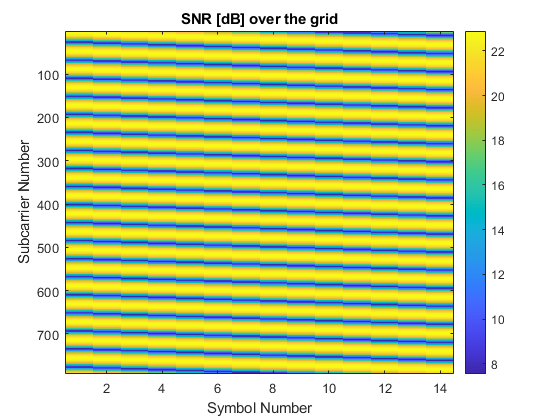
\includegraphics[width=\maxwidth{56.196688409433015em}]{figure_1.png}
\end{center}


\begin{par}
\begin{flushleft}
We will now look at the average SNR over different slots.   Suppose we transmit on \texttt{slotNum=0} for \texttt{sfNum=i} for \texttt{i=0,...,ntx} for \texttt{ntx=100. } Hence, we are transmitting once per subframe.  For each transmission, compute the channel and the average SNR.  Plot the average SNR as a function of the transmission number.  You should see that it is very constant.  Thus, although individual resource elements are fading, the average SNR experienced over different blocks indicating that there is \textbf{neglible} \textbf{slow fading}.  
\end{flushleft}
\end{par}

\begin{matlabcode}
% TODO
ntx = 100;
slotNum = 0;
avgSNRs = zeros(ntx+1,1);
for j=1:ntx+1
    [~, chanGrid_sf, noiseVar_sf] = fdchan.step(txGrid, j-1, slotNum);
    SNR = mean((abs(chanGrid_sf).^2 / noiseVar_sf),"all");
    avgSNRs(j) = pow2db(SNR);
end

figure;
plot(0:ntx, avgSNRs, "LineWidth",2);
xlabel("Subframe Number"); ylabel("Avg SNR [dB]"); grid on;
title("Avg SNR for each transmission number"); ylim([19.9, 20.1]);
\end{matlabcode}
\begin{center}
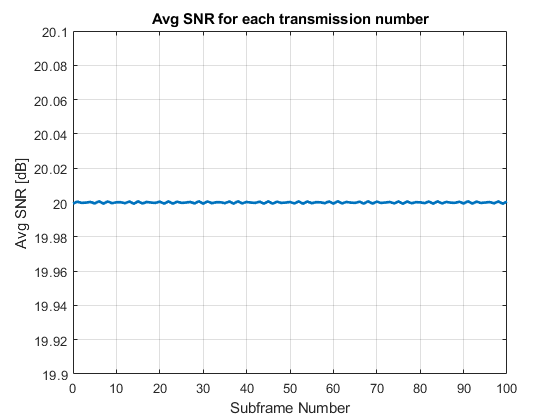
\includegraphics[width=\maxwidth{56.196688409433015em}]{figure_2.png}
\end{center}


\matlabheading{Creating a Simple NR PDSCH Transmitter}


\vspace{1em}
\begin{par}
\begin{flushleft}
Downlink data (the link from the base station to the UE) in the NR system is transmitted on what is called the PDSCH channel or Physical Downlink Shared Channel.  It is called \textit{shared} since multiple UEs share the channel.  Each transmissions is called a transport block.  The transport block occupies one slot with a variable number of resource blocks.  Multiple UEs can be scheduled in the slot on different resource blocks.  When we discuss MIMO technologies, users will also be able to be transmitted on different \textit{streams} or layers, but for now we will just use a single antenna system with one layer.
\end{flushleft}
\end{par}

\begin{par}
\begin{flushleft}
Each transport block has one of 28 \textbf{modulation and coding scheme (MCS) }given by this table.
\end{flushleft}
\end{par}

\begin{par}
\begin{flushleft}
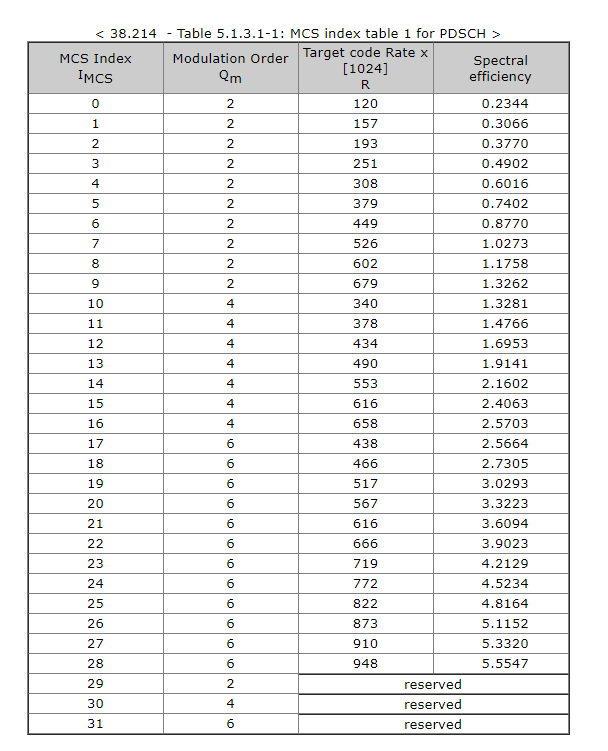
\includegraphics[width=\maxwidth{-0.10035122930255896em}]{image_3}
\end{flushleft}
\end{par}

\begin{par}
\begin{flushleft}
For this simulation we will use MCS=13.  
\end{flushleft}
\end{par}

\begin{matlabcode}
mcsInd = 13;

% TODO
Modulation = '16QAM'; % MCS 13 is 4 bits per symbol
targetCodeRate = 490/1024;
\end{matlabcode}

\begin{par}
\begin{flushleft}
Once you have selected these parameters, we can confgure the PDSCH transmission with the following command.  In this case, I have configured the PDSCH to use all the RBs and all but the first OFDM symbol in a slot.  I have also added what is called the phase tracking reference signal (PTRS) for mitigating phase noise.  We will discuss this channel more later when we disucss equalaization.
\end{flushleft}
\end{par}

\begin{matlabcode}
pdschConfig = nrPDSCHConfig(...
    'Modulation', Modulation, ...
    'PRBSet', (0:NRB-1), ...
    'SymbolAllocation', [1, waveformConfig.SymbolsPerSlot-1], ...
    'EnablePTRS', 1,...
    'PTRS', nrPDSCHPTRSConfig());
\end{matlabcode}


\begin{par}
\begin{flushleft}
The NR has an extremely complex way of transmitting data involving LDPC encoding, scrambling, mapping to QAM symbols and then placing the symbols on the RX grid.  These would takes months of time to write from scratch.  The 5G toolbox has amazing functions to do all of this for you.  
\end{flushleft}
\end{par}

\begin{par}
\begin{flushleft}
I have created a simple TX class using these functions.  You will not need to modify it.  But, we will just look at the outputs.  You can create an instance of this class as follows.
\end{flushleft}
\end{par}

\begin{matlabcode}
tx = NRgNBTxFD(carrierConfig, pdschConfig, 'targetCodeRate', targetCodeRate);
\end{matlabcode}


\begin{par}
\begin{flushleft}
You can then call the \texttt{step} method to generate random bits for one slot of data based on the PDSCH configuration.  If you look at the code in the step implementation you can see the MATLAB 5G Toolbox commands to encode and modulate the data.
\end{flushleft}
\end{par}

\begin{matlabcode}
txGrid = tx.step();
\end{matlabcode}


\begin{par}
\begin{flushleft}
Use the \texttt{imagesc} command to plot the set of resource elements in the grid where \texttt{txGrid} is non-zero.  These are the resource elements (REs) where the PDSCH channel is allocated.  You should see that the PDSCH is allocated except at the following locations:
\end{flushleft}
\end{par}

\begin{itemize}
\setlength{\itemsep}{-1ex}
   \item{\begin{flushleft} The first OFDM symbol.  This is where the assignment channel, called the PDCCH, will go.  Basically this communicates to the UEs the resource allocation, UE identity in that slot.  We will discuss \end{flushleft}}
   \item{\begin{flushleft} The third OFDM symbol. which is used as demodulation reference signal (DM-RS) used in channel estimation.  We will discuss this when we discuss equalization \end{flushleft}}
   \item{\begin{flushleft} The horizontal strips.  These are PT-RS for phase noise mitigation that we will also discuss later. \end{flushleft}}
\end{itemize}

\begin{matlabcode}
% TODO
figPos = get(0,'defaultfigureposition');
width = 1e3;
height = 1e3;
figure('Position', [figPos(1), figPos(2), width, height]);
reGrid = zeros(size(txGrid));
reGrid(abs(txGrid) ~= 0) = 1;
imagesc(1:14, 1:nsc, uint8(reGrid));
xlabel("Symbol Number"); ylabel("Subcarrier Number");
colorbar();
\end{matlabcode}
\begin{center}
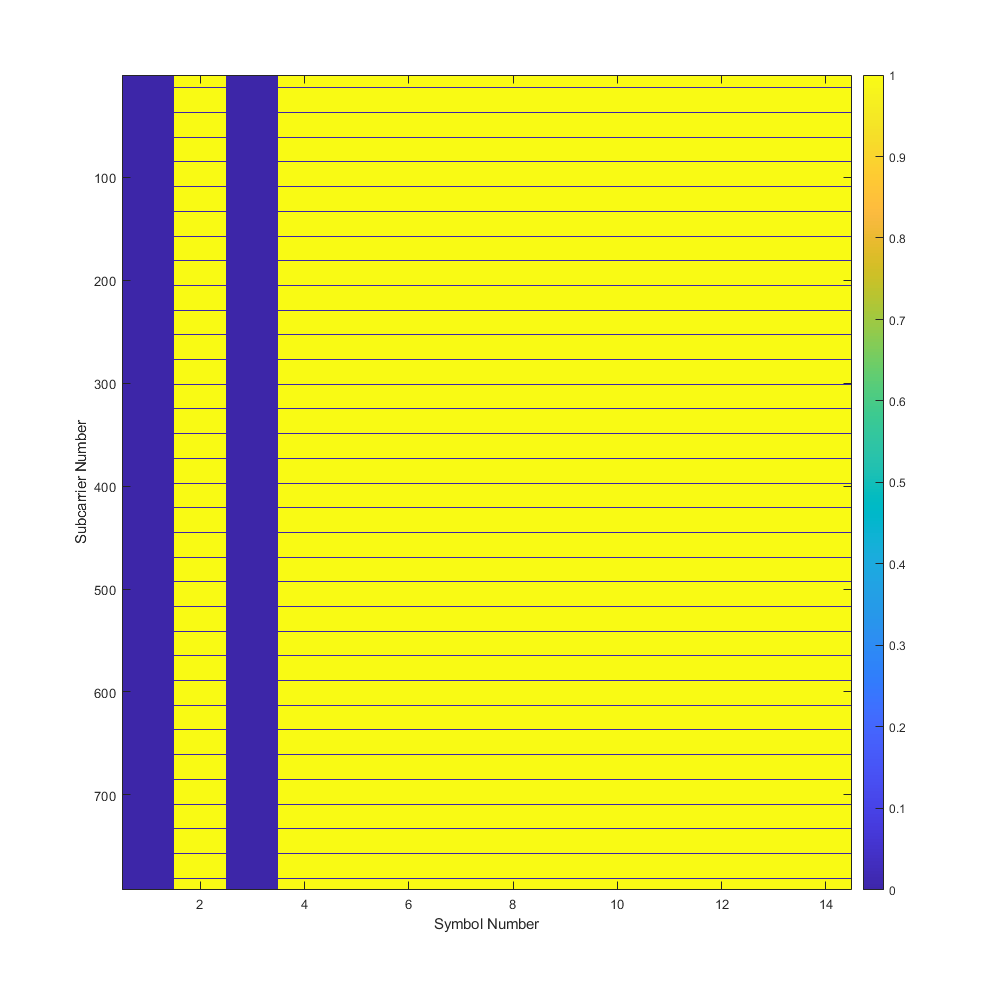
\includegraphics[width=\maxwidth{80.28098344204717em}]{figure_3.png}
\end{center}
\begin{matlabcode}
% We can see that the first and third OFDM symbols across all subcarriers
% are occupied (by the PDCCH and DM-RS respectively)
% We can also see the horizontal strips
\end{matlabcode}


\begin{par}
\begin{flushleft}
Next, compute and print:
\end{flushleft}
\end{par}

\begin{itemize}
\setlength{\itemsep}{-1ex}
   \item{\begin{flushleft} The number of REs allocated to the PDSCH in the slot \end{flushleft}}
   \item{\begin{flushleft} The fraction of PDSCH REs to the total number of REs. \end{flushleft}}
\end{itemize}

\begin{matlabcode}
% TODO
reSlot = reGrid(:,4); 
nREPdsch = sum(reSlot)*12;
bwFrac = sum(reGrid,"all")/(NRB*12*14);

fprintf(1, 'The number of REs allocated in one slot = %.f\n', nREPdsch);
\end{matlabcode}
\begin{matlaboutput}
The number of REs allocated in one slot = 9108
\end{matlaboutput}
\begin{matlabcode}
fprintf(1, 'The fraction of PDSCH REs to the total number of REs = %.6f\n', bwFrac);
\end{matlabcode}
\begin{matlaboutput}
The fraction of PDSCH REs to the total number of REs = 0.821429
\end{matlaboutput}


\begin{par}
\begin{flushleft}
Next, let's look at the transmitted QAM symbols.  The NR standard has a complex mapping of the PDSCH to the REs..  We can use the following command to get the indices, \texttt{pdschInd},  of the PDSCH locations for a given configuraiton.  It also returns a structure, \texttt{pdschInfo} with other modualtion data.
\end{flushleft}
\end{par}

\begin{matlabcode}
% Get indices on where the PDSCH is allocated
[pdschInd,pdschInfo] = nrPDSCHIndices(carrierConfig, pdschConfig);
\end{matlabcode}

\begin{par}
\begin{flushleft}
Use the PDSCH symbols from \texttt{txGrid} from the \texttt{pdschInd} and plot the resulting constellation diagram.  You should see a 16-QAM constellation with unit average power.
\end{flushleft}
\end{par}

\begin{matlabcode}
% TODO
flat_txGrid = txGrid(:);
pdschSym = flat_txGrid(pdschInd);
plot(real(pdschSym), imag(pdschSym), 'o');
grid on; title("16-QAM constellation diagram of the tx symbols");
\end{matlabcode}
\begin{center}
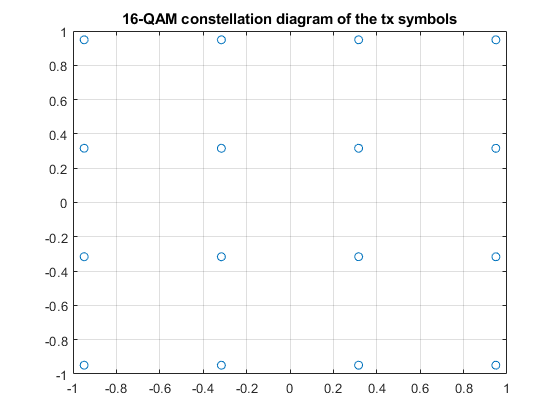
\includegraphics[width=\maxwidth{56.196688409433015em}]{figure_4.png}
\end{center}


\begin{par}
\begin{flushleft}
Finally, let's compute the spectral efficiency.  In NR, the transmitted information bits for a transport block can be stored in either one or two codewords.  For this configuration, there will only be one codeword (two codewords are used when there are more than four spatial streams).  The randomly generated information bits in the transmission are stored in a field, \texttt{tx.txBits\{1\}.  }Compute and print:
\end{flushleft}
\end{par}

\begin{itemize}
\setlength{\itemsep}{-1ex}
   \item{\begin{flushleft} The number of information bits that were transmitted in this transport block. \end{flushleft}}
   \item{\begin{flushleft} The spectral efficiency, meaning the number of information bits per PDSCH RE. \end{flushleft}}
\end{itemize}

\begin{par}
\begin{flushleft}
The spectral efficiency should be close to the target spectral efficiency in the MCS table.
\end{flushleft}
\end{par}

\begin{matlabcode}
% TODO
txbits = tx.txBits{1};
n_info_bits = length(txbits);
tot_bits = nREPdsch*4;
se = n_info_bits/tot_bits*4;
fprintf(1, 'The number of information bits in the TB = %.f\n', n_info_bits);
\end{matlabcode}
\begin{matlaboutput}
The number of information bits in the TB = 17424
\end{matlaboutput}
\begin{matlabcode}
fprintf(1, 'The spectral efficiency = %.6f\n', se);
\end{matlabcode}
\begin{matlaboutput}
The spectral efficiency = 1.913043
\end{matlaboutput}


\matlabheading{Building an NR Receiver}

\begin{par}
\begin{flushleft}
We will next build a simple NR receiver at the UE.  I have written most of the code containe in a class \texttt{NRUERxFD}.    However, there are a few sections labeled \texttt{TODO} in the \texttt{stepImpl} method.  These just call built-in functions from the 5G Toolbox for equalization, LLR computation and decoding.  You just need to supply each function with the correct inputs.   
\end{flushleft}
\end{par}

\begin{par}
\begin{flushleft}
Once you have completed the \texttt{TODO} parts, an RX object can be created as follows.
\end{flushleft}
\end{par}

\begin{matlabcode}
% rx = NRUERxFD(carrierConfig, pdschConfig, 'targetCodeRate', targetCodeRate);
\end{matlabcode}


\begin{par}
\begin{flushleft}
Now test the receiver:
\end{flushleft}
\end{par}

\begin{itemize}
\setlength{\itemsep}{-1ex}
   \item{\begin{flushleft} Create a \texttt{NRgNBTxFD} transitter object, \texttt{tx} as above.   \end{flushleft}}
   \item{\begin{flushleft} Run the TX to create one slot of symbols. \end{flushleft}}
   \item{\begin{flushleft} Create an \texttt{FDChan} object as above with the two paths and an average SNR of 20 dB. \end{flushleft}}
   \item{\begin{flushleft} Run the \texttt{txGrid} through the chanel at slot = 0 and subframe = 0 \end{flushleft}}
   \item{\begin{flushleft} Create a RX object, \texttt{rx} of type \texttt{NRUERxFD.} \end{flushleft}}
   \item{\begin{flushleft} Run the RX grid, channel grid and noise variance into the RX \end{flushleft}}
   \item{\begin{flushleft} Make sure that \texttt{rx.rxBits == tx.txBits\{1\}}.   \end{flushleft}}
\end{itemize}

\begin{matlabcode}
% TODO:  Create the TX
tx = NRgNBTxFD(carrierConfig, pdschConfig, 'targetCodeRate', targetCodeRate);
txGrid = tx.step();
fdchan = FDChan(waveformConfig, 'gain', gain, 'dly', dly, 'aoaAz', aoaAz, 'aoaEl', aoaEl, ...
                'rxVel', rxVel, 'Etx', Etx, 'EsN0Avg', 20, 'fc', fc);
[rxGrid, chanGrid, noiseVar] = fdchan.step(txGrid, 0, 0);
rx = NRUERxFD(carrierConfig, pdschConfig, 'targetCodeRate', targetCodeRate);
rx.step(rxGrid, chanGrid, noiseVar);
rxBits = rx.rxBits;
txBits = tx.txBits{1};
checkBits = sum(rxBits == txBits);

if checkBits == length(txBits)
    disp("All bits received correctly");
end
\end{matlabcode}
\begin{matlaboutput}
All bits received correctly
\end{matlaboutput}


\begin{par}
\begin{flushleft}
Also, plot the equalization constelllation stored in the RX.
\end{flushleft}
\end{par}

\begin{matlabcode}
% TODO
figure;
plot(real(rx.pdschEq), imag(rx.pdschEq), 'o');
title("Equalized Rx Symbols"); grid on;
\end{matlabcode}
\begin{center}
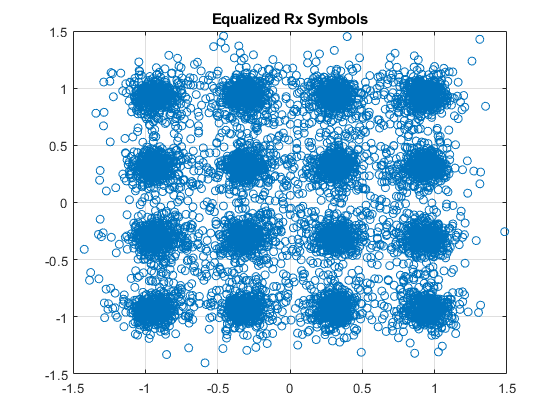
\includegraphics[width=\maxwidth{56.196688409433015em}]{figure_5.png}
\end{center}


\matlabheading{Testing the Receiver Performance}

\begin{par}
\begin{flushleft}
The above validated the performance of the RX at high SNR.  Now vary the SNR, \texttt{EsN0Avg} from 5 to 10 dB in 1 dB steps.  In each SNR, simulate the link above with repeated transmissions one subframe apart.  At each SNR, repeat until either:
\end{flushleft}
\end{par}

\begin{itemize}
\setlength{\itemsep}{-1ex}
   \item{\begin{flushleft} You get 50 block errors, or \end{flushleft}}
   \item{\begin{flushleft} You have tested at least 500 TX \end{flushleft}}
\end{itemize}

\begin{par}
\begin{flushleft}
Once you have a SNR with zero block errors, you can stop and not continue to the higher SNRs.  Measure the block error rate at each SNR.  This may take a few minutes.
\end{flushleft}
\end{par}

\begin{par}
\begin{flushleft}
Plot the BLER vs. SNR.  If you do everything correctly, you should get that the BLER goes to zero Es/N0=8 dB.
\end{flushleft}
\end{par}


\vspace{1em}
\begin{matlabcode}
% TODO:  Compute BLER vs. EsN0Avg
EsN0Avg_values = 5:10;
tx = NRgNBTxFD(carrierConfig, pdschConfig, 'targetCodeRate', targetCodeRate);
rx = NRUERxFD(carrierConfig, pdschConfig, 'targetCodeRate', targetCodeRate);
max_tx = 500;
max_be = 50;
BLER = zeros(length(EsN0Avg_values), 1);

for i=1:length(EsN0Avg_values)
    EsN0Average = EsN0Avg_values(i);
    fdchan = FDChan(waveformConfig, 'gain', gain, 'dly', dly, 'aoaAz', aoaAz, 'aoaEl', aoaEl, ...
                    'rxVel', rxVel, 'Etx', Etx, 'EsN0Avg', EsN0Average, 'fc', fc);
    subF_num = 0;
    num_be = 0;
    while (subF_num < max_tx) && (num_be < max_be)  
        txGrid = tx.step();
        [rxGrid, chanGrid, noiseVar] = fdchan.step(txGrid, subF_num, 0);
        rx.step(rxGrid, chanGrid, noiseVar);
        rxBits = rx.rxBits;
        txBits = tx.txBits{1};
        checkBits = sum(rxBits == txBits);

        if checkBits ~= length(txBits)
            num_be = num_be+1;
        end
        subF_num = subF_num+1;
    end 
    
    BLER(i) = num_be / (subF_num);
    fprintf(1, 'EsN0 = %.6f\n', EsN0Average);
    fprintf(1, 'BLER = %.6f\n', BLER(i));
    if num_be == 0
        disp("Zero block errors in 500 txs: stopping");
        break;
    end
end
\end{matlabcode}
\begin{matlaboutput}
EsN0 = 5.000000
BLER = 1.000000
EsN0 = 6.000000
BLER = 1.000000
EsN0 = 7.000000
BLER = 1.000000
EsN0 = 8.000000
BLER = 0.000000
Zero block errors in 500 txs: stopping
\end{matlaboutput}


\begin{matlabcode}
% TODO:  Plot BLER vs EsN0Avg
figure;
plot(EsN0Avg_values, BLER, 'o-', "LineWidth",2); grid on;
xlabel("EsN0Avg [dB]"); ylabel("BLER");
title("BLER vs EsN0Avg");
\end{matlabcode}
\begin{center}
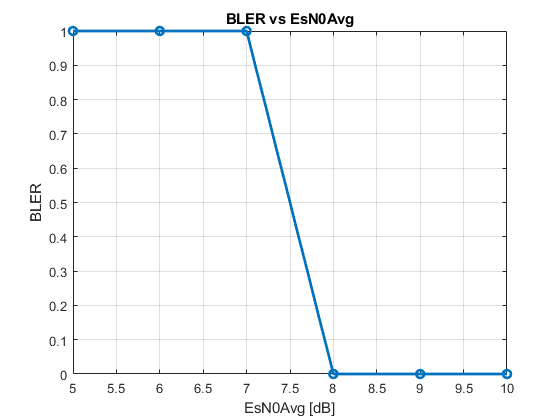
\includegraphics[width=\maxwidth{56.196688409433015em}]{figure_6.png}
\end{center}


\matlabheading{Estimating the Shannon Ergodic Capacity}

\begin{par}
\begin{flushleft}
We conclude by estimating the theoretical Shannon capacity over a typical slot.  The Shannon ergodic spectral efficiency is:
\end{flushleft}
\end{par}

\begin{verbatim}
seShannon = mean( log2( 1 + c*gamma) )
c = abs(chanGrid).^2 / mean(abs(chanGrid).^2)
\end{verbatim}
\begin{par}
\begin{flushleft}
where \texttt{chanGrid} are the complex channel gains on the OFDM grid and gamma is the average Es/N0.
\end{flushleft}
\end{par}

\begin{par}
\begin{flushleft}
Compute this Shannon spectral efficiency vs. EsN0 for 0 to 10 dB.  You should see that theoretically, you can achieve the spectral efficiency in the MCS of 1.9 bps/Hz at about Es/N0 = 5.3 dB.  So, the NR code only runs about 2 to 2.5 dB below Shannon capacity.
\end{flushleft}
\end{par}


\vspace{1em}
\begin{matlabcode}
% TODO
npoints = 100;
EsN0 = linspace(0,10,npoints);
c = abs(chanGrid(:)).^2;
c = c / mean(c);
seShannon = zeros(npoints,1);
for i=1:npoints
    seShannon(i) = mean(log2(1 + c*db2pow(EsN0(i))));
end

EsN0_shannon = interp1(seShannon,EsN0,se);
figure;
plot(EsN0, seShannon, "LineWidth",2); grid on;
hold on;
plot(repelem(EsN0_shannon, npoints), linspace(0.5,3.5,npoints), "k-")
hold off; xlabel("EsN0 [dB]"); ylabel("SE [bits/sec/Hz]");
legend("Shannon SE","Min SNR for 1.91 se (MSC 13)");
\end{matlabcode}
\begin{center}
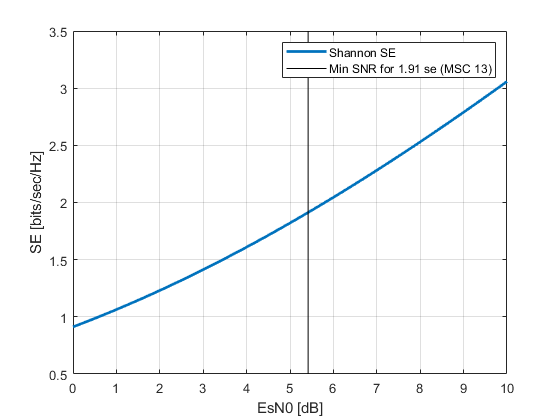
\includegraphics[width=\maxwidth{56.196688409433015em}]{figure_7.png}
\end{center}
\begin{matlabcode}

\end{matlabcode}

\end{document}
